% Options for packages loaded elsewhere
\PassOptionsToPackage{unicode}{hyperref}
\PassOptionsToPackage{hyphens}{url}
%
\documentclass[
  8pt]{extarticle}
\usepackage{amsmath,amssymb}
\usepackage{iftex}
\ifPDFTeX
  \usepackage[T1]{fontenc}
  \usepackage[utf8]{inputenc}
  \usepackage{textcomp} % provide euro and other symbols
\else % if luatex or xetex
  \usepackage{unicode-math} % this also loads fontspec
  \defaultfontfeatures{Scale=MatchLowercase}
  \defaultfontfeatures[\rmfamily]{Ligatures=TeX,Scale=1}
\fi
\usepackage{lmodern}
\ifPDFTeX\else
  % xetex/luatex font selection
\fi
% Use upquote if available, for straight quotes in verbatim environments
\IfFileExists{upquote.sty}{\usepackage{upquote}}{}
\IfFileExists{microtype.sty}{% use microtype if available
  \usepackage[]{microtype}
  \UseMicrotypeSet[protrusion]{basicmath} % disable protrusion for tt fonts
}{}
\makeatletter
\@ifundefined{KOMAClassName}{% if non-KOMA class
  \IfFileExists{parskip.sty}{%
    \usepackage{parskip}
  }{% else
    \setlength{\parindent}{0pt}
    \setlength{\parskip}{6pt plus 2pt minus 1pt}}
}{% if KOMA class
  \KOMAoptions{parskip=half}}
\makeatother
\usepackage{xcolor}
\usepackage{graphicx}
\makeatletter
\def\maxwidth{\ifdim\Gin@nat@width>\linewidth\linewidth\else\Gin@nat@width\fi}
\def\maxheight{\ifdim\Gin@nat@height>\textheight\textheight\else\Gin@nat@height\fi}
\makeatother
% Scale images if necessary, so that they will not overflow the page
% margins by default, and it is still possible to overwrite the defaults
% using explicit options in \includegraphics[width, height, ...]{}
\setkeys{Gin}{width=\maxwidth,height=\maxheight,keepaspectratio}
% Set default figure placement to htbp
\makeatletter
\def\fps@figure{htbp}
\makeatother
\setlength{\emergencystretch}{3em} % prevent overfull lines
\providecommand{\tightlist}{%
  \setlength{\itemsep}{0pt}\setlength{\parskip}{0pt}}
\setcounter{secnumdepth}{-\maxdimen} % remove section numbering
% --- Preamble for Cheatsheet ---
\usepackage[a4paper, landscape, margin=0.5cm]{geometry} % 设置 A4 横向,边距 1cm
\usepackage{amsmath}          % 数学公式增强
\usepackage{amssymb}          % 数学符号 (如 \mathbb)
\usepackage{graphicx}         % 支持插入图片
\usepackage{multicol}         % 支持多栏排版
\setlength{\columnsep}{1em}    % 设置栏间距
\usepackage{parskip}          % 使用段落间距代替首行缩进,更紧凑
\setlength{\parskip}{0.5em plus 0.1em minus 0.1em}
\setlength{\parindent}{0pt}
\usepackage{ctex}             % ctex 中文支持
\graphicspath{{source/}}


% 可选:如果默认字体不满意,可以取消注释并指定字体
% \setmainfont{Noto Serif CJK SC}
% \setsansfont{Noto Sans CJK SC}
% \setmonofont{Noto Sans Mono CJK SC}

\setcounter{secnumdepth}{2}    % 可选:控制章节编号深度,Cheatsheet 可能不需要太深
% --- End Preamble ---
\ifLuaTeX
  \usepackage{selnolig}  % disable illegal ligatures
\fi
\IfFileExists{bookmark.sty}{\usepackage{bookmark}}{\usepackage{hyperref}}
\IfFileExists{xurl.sty}{\usepackage{xurl}}{} % add URL line breaks if available
\urlstyle{same}
\hypersetup{
  hidelinks,
  pdfcreator={LaTeX via pandoc}}

\author{}
\date{}

\begin{document}

\begin{multicols*}{4}
    \footnotesize

    \begin{center}
        \textbf{CV Cheatsheet} by 卓致用\ 徐靖\ 陈佳伟\ 李柏睿\ 何劲范
    \end{center}
    \vspace{-1.75em} % 减少标题与内容的间距

\hypertarget{d-vision}{%
\section{3D Vision}\label{d-vision}}

\textbf{PointNet++}:一个很 General 的模型,它甚至可以用在 MNIST
上(做数字分类)。在分类问题上,PointNet++是 \textbf{各向同性 Isotropic}
的(无法区分邻域点在不同相对位置上的信息),而 Conv 是 \textbf{各向异性
Anisotropic} 的。改进:HyerNetworks/KP-Conv 线性插值,但都烂。

\textbf{Voxelization (体素化)}:天然各向异性,将点云转换为 3D
体素网格,使用 4D 核(DHWC)进行 3D
卷积。\textbf{优点}:高效,支持索引,与 2D
卷积一样具有表现力、平移不变性。\textbf{问题}:贵。早期模型输入分辨率低(如
\(30^3\)),\textbf{离散误差(Discretization
error)}即点云到体素的误差导致信息丢失,但可以存一下原始点云 avg local
feature 进去。\textbf{Sparse Voxel}:只在表面占据格点。

\textbf{Sparse Convolution
(稀疏卷积)}:体素化中大部分网格为空,故只存储和计算非零体素(表面信号)及其邻域的卷积(这种稀疏存储的体素数量甚至可能比原始点云的点数还要少,因为一个体素内可能包含多个点),输出也是稀疏的。\textbf{优点}:效率远高于密集卷积;Voxel
是可索引的规则网络;与 2D Conv
相似的表达能力和平移不变性。\textbf{缺点}:离散误差。

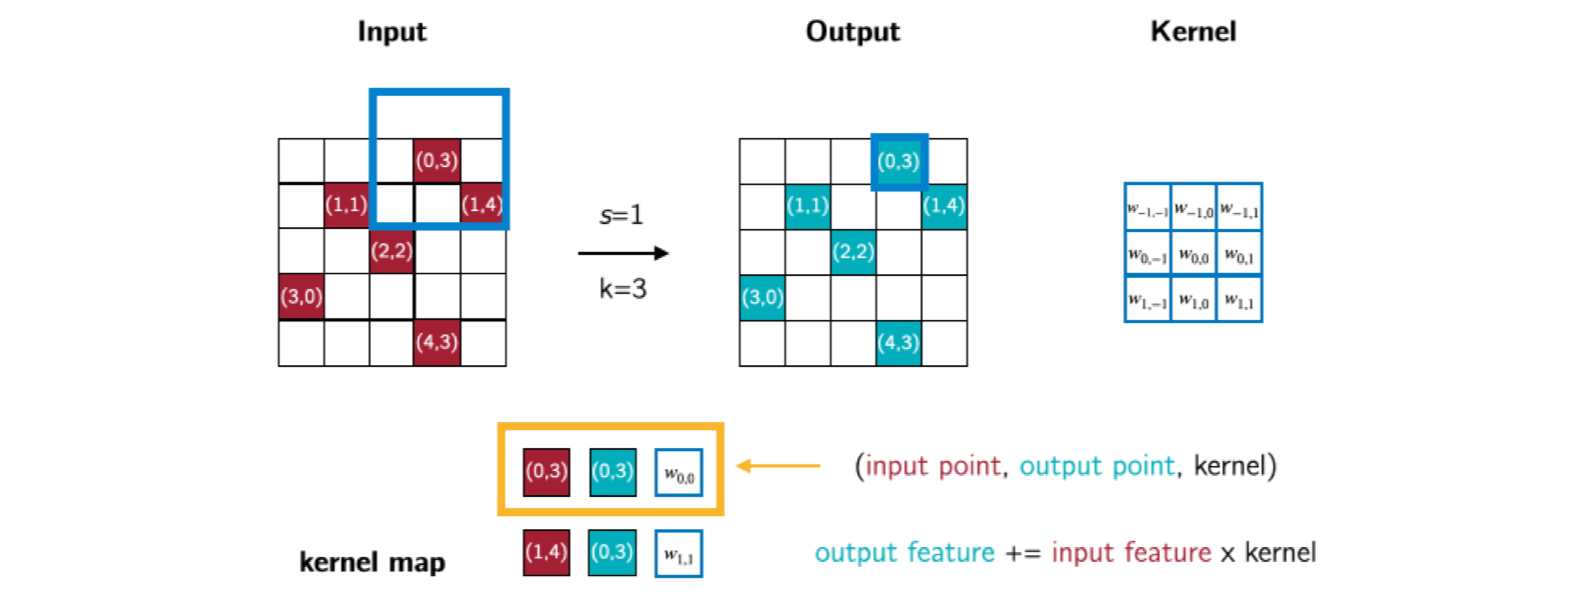
\includegraphics{./Cheatsheet-01-Sequential-Data.assets/image-20250618022954153.png}

\textbf{稀疏卷积 vs.~点云网络}:1. \textbf{分辨率}:PCN
更高、细节更精细(但不一定就更好),SC 受限。 2. \textbf{各向性}:PCN
各向同性,SC 各向异性。 3. \textbf{效率}:SC 索引和邻域查询更高效,PCN
的 FPS 和球形查询较慢。 4. \textbf{易用性}:PCN
更易用,适合作为初步选择。 5. \textbf{场景规模}:SC
适用于大规模场景如激光雷达,PCN 性能略低、适用于小尺度精细场景如灵巧手。

\hypertarget{sequential-data}{%
\section{Sequential Data}\label{sequential-data}}

\textbf{序列数据处理模式}:与顺序无关的点云不同,序列数据的顺序至关重要。

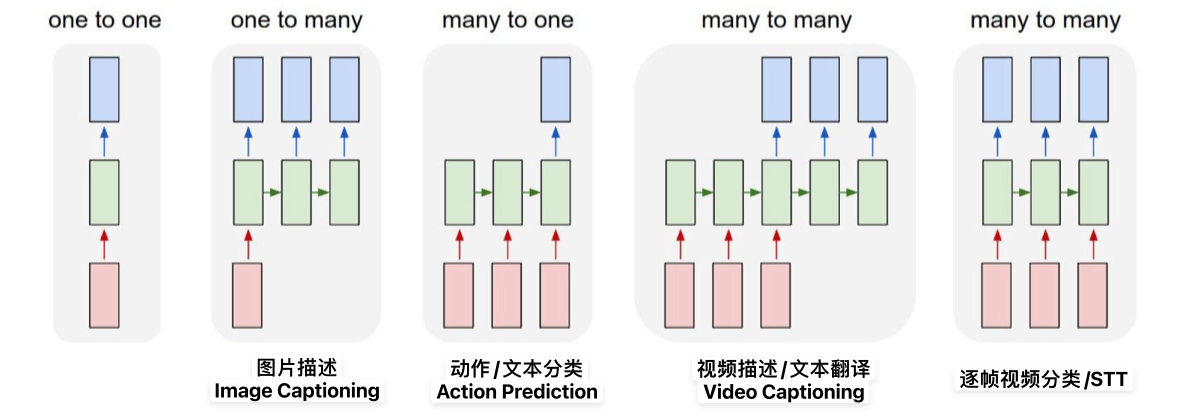
\includegraphics{./Cheatsheet-01-Sequential-Data.assets/image-20250617211140565.png}

\textbf{RNN 核心思想}:关键在 \textbf{隐藏状态 (Hidden State)}
\(h\),它作为记忆单元,随序列输入不断更新。迭代:\(h_t = f_W(h_{t-1}, x_t)\)。\textbf{权重共享}:权重
\(W\)
在所有时间步复用,使得模型能处理任意长度的序列,且对输入具有一定\textbf{对称性
Symmetry}。在每个时间步,可根据当前隐藏状态计算输出
\(y_t = f_{W_{hy}}(h_t)\)。

\textbf{Vanilla RNN}:\(h_t=\tanh(W_{hh}h_{t-1}+W_{xt}x_t)\),
\(y_t=W_{hy}h_t\)。每个输出 \(y_t\) 产生一个损失 \(L_t\),总损失
\(L=\sum L_t\)。计算量大,通常只在序列块(chunk)上反向传播(BPTT)。\textbf{优势}:1.RNN能以固定的参数量处理任意长度的输入;2.利用多步之前的信息;3.
在每个时间步上应用相同的权重,因此输入处理方式是等变的;4.模型大小不会因输入长度变长而增加。\textbf{劣势}:1.
循环计算很慢;2. 远距离的梯度信号容易丢失。

\textbf{BPTT (Backpropagation Through Time)}:由于权重 \(W\)
共享,最终作用于 \(W\) 的总梯度是所有时间步的损失回传到 \(W\)
的梯度之和。\textbf{Truncated BPTT}:对于长序列,完整 BPTT
需巨大的计算/内存开销,故截断出反向传播的序列长度形成 chunks
\(\Delta T\) ,前向正常或每块初始部分都置为
\(h_0\)(序列过长时),反向只在窗口内计算、更新。若输入置为
\(h_0\),则同时限制了模型学习长期依赖的能力(换取计算可行性的代价)。

\textbf{Character-Level Language Model Sampling}:将当前步输出 \(y_t\)
作为下一步输入 \(x_{t+1}\) 以生成序列。\textbf{Greedy
sampling}:总是选概率最高的 token,完全确定性。\textbf{Weighted
sampling}:按概率分布采样,更多样但可能采样出错导致后续崩盘。\textbf{Beam
Search}:在每个时间步保留 \(k\) 个最可能的序列,作为一种介于贪心和
\(O(V^T)\) 的穷举搜索 \textbf{Exhaustive Search}
\(P(y|x) = \prod_{t=1}^{T} P(y_t | y_{<t}, x)\)
之间的策略,平衡效果与效率,\textbf{不保证找到全局最优解}。

\textbf{Embedding Layer}:在输入层和隐藏层之间加入,将 one-hot
向量映射为稠密向量,通常不参与反向传播。

\textbf{RNN
梯度问题}:\(\frac{\partial h_t}{\partial h_{t-1}} = \tanh'(W_{hh} h_{t-1} + W_{xh} x_t) W_{hh}\),\(\frac{\partial L_T}{\partial W} = \frac{\partial L_T}{\partial h_T} \left( \prod_{t=2}^{T} \frac{\partial h_t}{\partial h_{t-1}} \right) \frac{\partial h_1}{\partial W}\),\(\frac{\partial L}{\partial W} = \sum_{t=1}^{T} \frac{\partial L_t}{\partial W}\),因反传时
tanh 梯度恒在 \((0, 1]\) ,易出现梯度消失。若无非线性激活,则变为
\(\frac{\partial L_T}{\partial W} = \frac{\partial L_T}{\partial h_T} W_{hh}^{T-1} \frac{\partial h_1}{\partial W}\),梯度由权重矩阵
\(W\) 的最大奇异值决定(大于 1 则爆炸,小于 1 则消失)。\textbf{Gradient
Clipping}:缩放梯度(范数超过阈值则除范数缩放到阈值)来处理梯度爆炸问题,但无法解决梯度消失(RNN
更本质的问题)。

\textbf{Multilayer RNN}:多层 RNN
堆叠,前一层的隐藏状态是后一层的输入,以增强非线性表达能力和特征提取。本身不解决长程依赖问题。

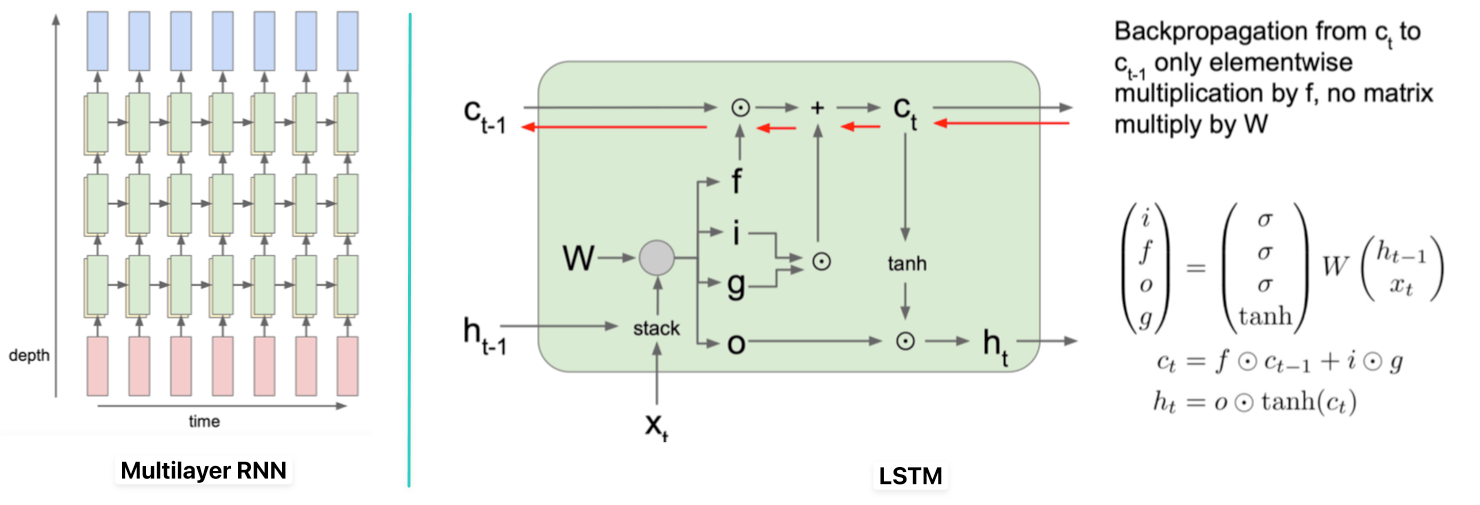
\includegraphics{./Cheatsheet-01-Sequential-Data.assets/image-20250617214406041.png}

\textbf{LSTM (Long-Short Term Memory)}:\textbf{记忆单元} \(c\)
存储和传递长期信息,\textbf{输入门} \(i\)
决定哪些新信息被存储,\textbf{遗忘门} \(f\)
决定哪些旧信息被遗忘,\textbf{输出门} \(o\)
决定从记忆单元中输出哪些信息,都用 \(\sigma\)
激活到\((0,1)\)。\textbf{候选门} \(g\) 用 \(\tanh\)
激活,取值\((-1,1)\),决定新信息的内容。\textbf{优点}:\textbf{LSTMs
不能保证解决梯度消失/爆炸问题,但能帮助学习长距离依赖关系}。当
\(f=1,\ i=0\) 时,单元信息 \(c\) 将一直保留。记忆单元 \(c\) 实现了
\textbf{skip-link} 的功能,为模型提供类似 ResNet 的效果。\textbf{GRU
(Gated Recurrent Unit)}:LSTM
的变体,合并了细胞状态和隐藏状态,门结构更简单,性能相当。

\textbf{加性互动(additive interaction)}:在反向传播时,从 \(c_t\) 传向
\(c_{t-1}\) 的梯度流非常直接,只经过一个逐元素的乘法(乘以遗忘门
\(f\)),而没有经过复杂的矩阵乘法和非线性激活函数的反复作用,从而可以缓解梯度消失,使得梯度可以几乎无衰减地长距离传播。

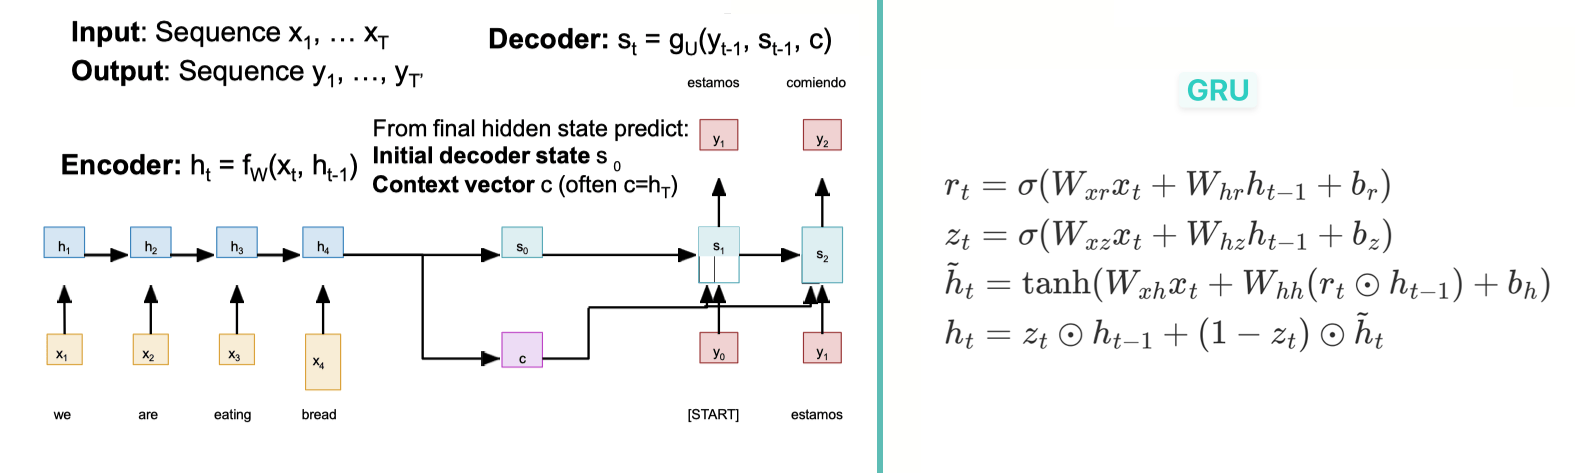
\includegraphics{./Cheatsheet-01-Sequential-Data.assets/image-20250618031316106.png}

\textbf{Encoder-Decoder 架构}:\textbf{编码器} 是一个
RNN,读取完整输入序列并压缩成一个固定大小的 \textbf{上下文向量
\(c\)},通常就是其最后一个隐藏状态。\textbf{解码器} 是另一个 RNN,接收
\(c\) 作为初始信息,并以自回归方式生成输出序列,状态更新
\(s_t = g(y_{t-1}, s_{t-1}, c)\),直到遇到终止符。

\textbf{信息瓶颈问题}:基本 Seq2Seq 架构要求将任意长度的输入压缩到
\textbf{固定大小} 的向量 \(c\)
中,当输入序列过长时,会造成信息损失,影响模型性能。

\textbf{Image Captioning}:多模态应用,使用 CNN
提取图像特征,将该特征作为 RNN
解码器的初始隐藏状态,生成描述图像的文本。\textbf{早期}:存在信息瓶颈,所有描述都必须从一个静态的图像特征中生成。\textbf{引入注意力机制}:编码器
CNN 提取图像的空间特征图(\(H \times W \times D\)),解码器 RNN
在生成每个词时,会计算当前隐藏状态对图像不同区域的注意力权重,动态聚焦于图像相关部分。

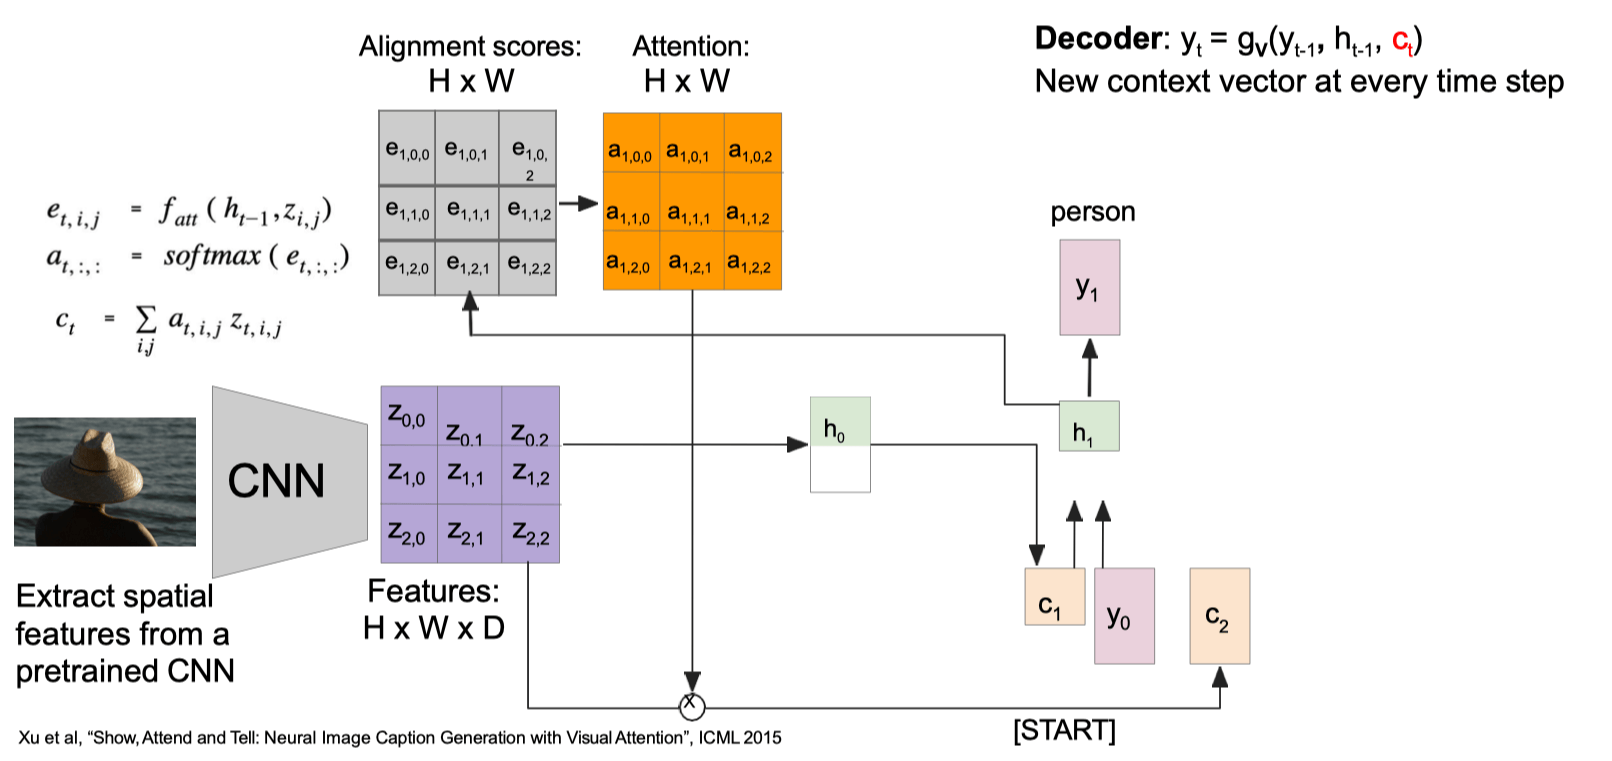
\includegraphics{./Cheatsheet-01-Sequential-Data.assets/image-20250617225104511.png}

\textbf{VQA (Visual Question Answering)}:多模态应用,分别用 CNN 和 RNN
提取图像和问题的特征,然后通过特征融合(如加法、逐元素乘法或拼接)来预测答案。确定最佳融合常依赖消融实验。\textbf{早期局限性}:1.
\textbf{图像特征的提取与问题完全独立},无法根据问题动态调整视觉注意力,即不同问题模型都使用相同的通用图像特征;2.
固定大小的上下文的瓶颈问题。

\hypertarget{attention-transformer}{%
\section{Attention \& Transformer}\label{attention-transformer}}

\textbf{Attention(RNN)}:将 QKV 映射到输出。Q 代表``要找什么'',K
代表``有什么信息'',V 代表``信息的具体内容''。通过计算 Q 和 K
的相似度得到权重(\(f_{att}\),MLP),再对 V
进行加权求和。注意力权重通常对每个 Query 按列进行 Softmax
归一化,使得一个 Query 对所有 Value 的关注度之和为
1。\textbf{公式}:\(e_{t,i} = f_{att}(s_{t-1}, h_i)\),\(\alpha_{t,i} = \frac{\exp(e_{t,i})}{\sum_{j=1}^{T} \exp(e_{t,j})}\),\(c_t = \sum_{i=1}^{T} \alpha_{t,i} h_i\),\(y_t = \text{Encoder}(c_t, y_{t-1})\)。\textbf{优点}:无消息瓶颈,每时间步动态获取上下文信息;端到端可微,自动学习无需对注意过程监督(模型自己领悟注意力权重);可解释性。

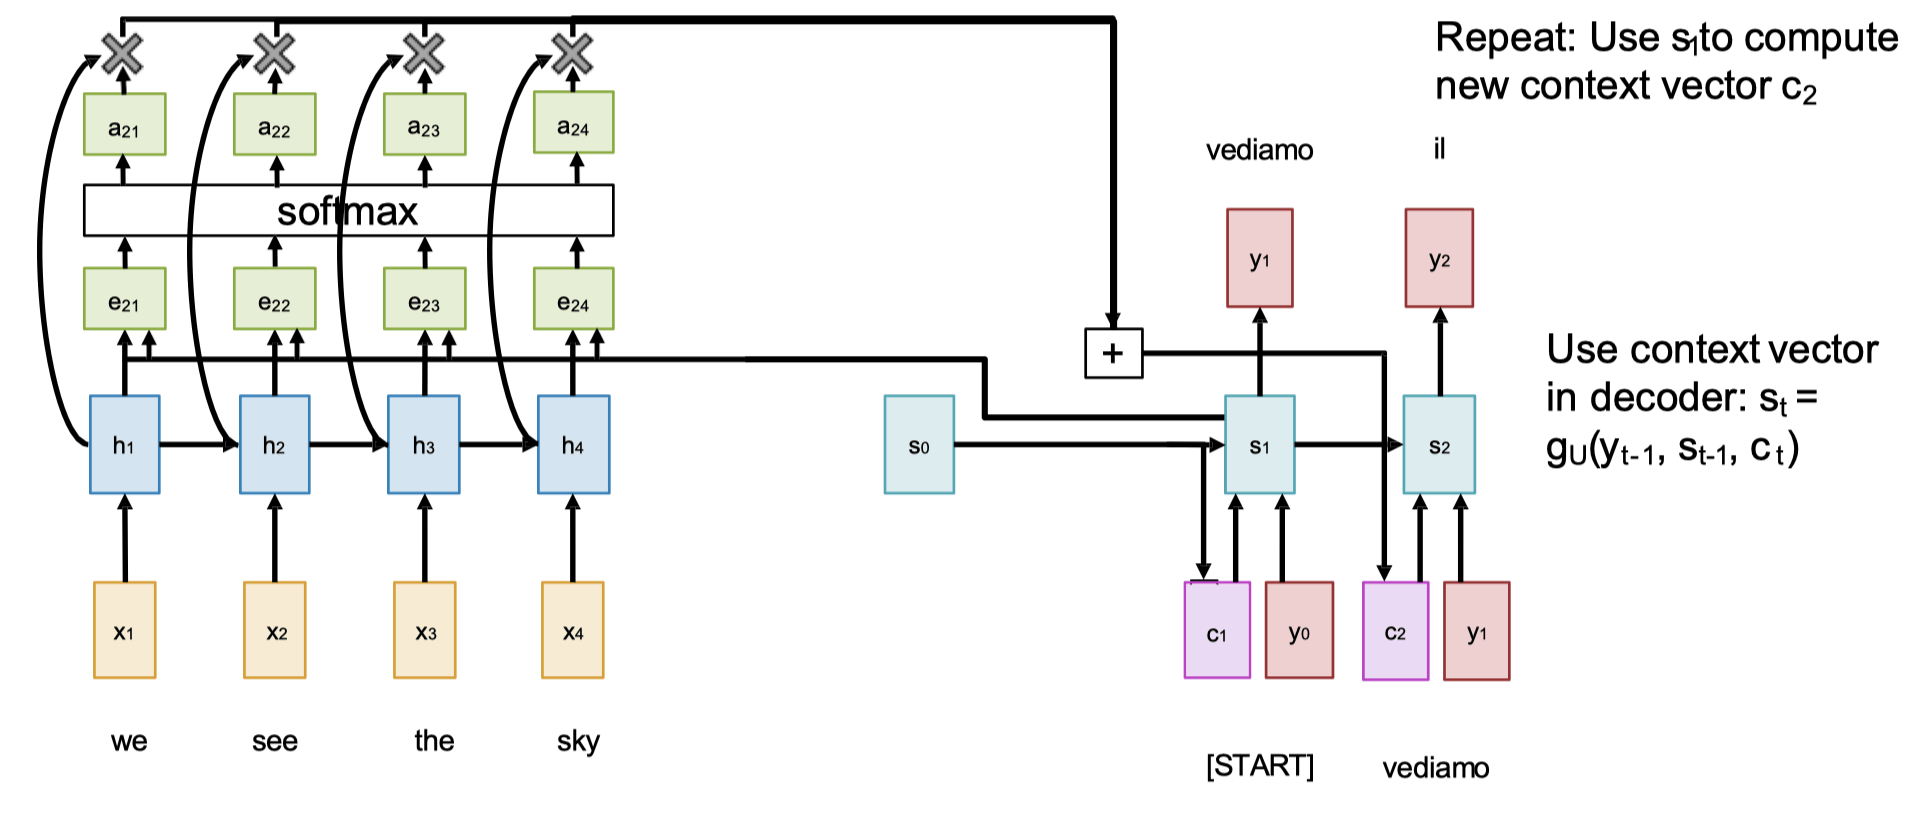
\includegraphics{./Cheatsheet-02-Self-Attention-and-Transformer.assets/image-20250618024935220.png}

\textbf{General Attention Layer}:1. \textbf{缩放点积}
\(\text{Attention}(Q, K, V) = \text{softmax}\left(\frac{QK^T}{\sqrt{d_k}}\right)V\);2.
\textbf{QKV 投影} \(K = XW_K\),\(V = XW_V\),\(Q = XW_Q\),这里的各处
\(X\) 可以相同(自注意力),也可以不同(交叉注意力),如 \(X_{Q}\)
可以是视觉特征,而 \(X_{K/V}\)
来自文本特征,再投影后便具有了同样的维度进行相关性计算,增加了模型的通用性。\textbf{对于
X 不变,对于 Q 置换等变。}

\textbf{为什么缩放}:当向量维度 \(d_k\)
很大时,点积的结果也可能变得非常大,导致 Softmax
函数进入饱和区(梯度接近于 0),使得梯度消失,模型难以训练。除以
\(\sqrt{d_k}\) 有效缩放,可以缓解。

\textbf{为什么将 X 做 KV 分开投影而不直接用 X}:是为了
\textbf{解耦两个核心功能}:\textbf{相关性计算(KQ)} 和
\textbf{信息聚合/提取(V)}。QK 和 V 可以具有不同维度。

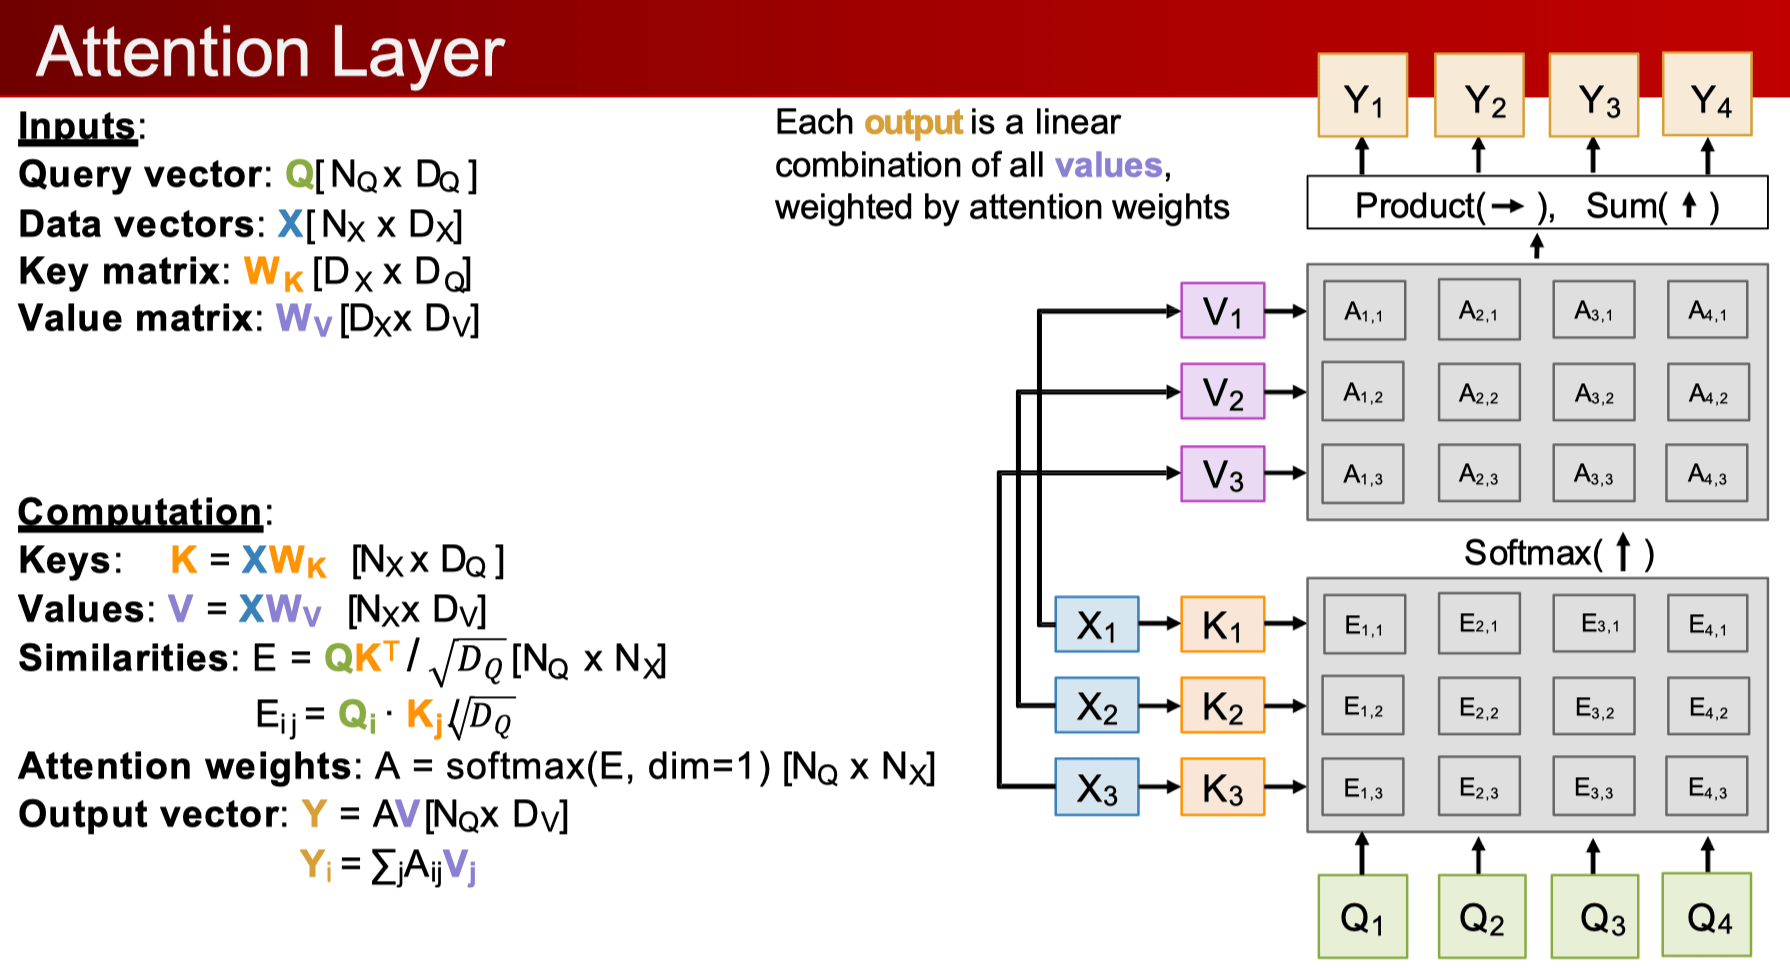
\includegraphics{./Cheatsheet-02-Self-Attention-and-Transformer.assets/image-20250617231033149.png}

\textbf{Self-Attention}:Attention 特例,其中 Q, K, V
均来自同一个输入序列 \(X_{Q}=X_{K}=X_{V}\)。相比
CNN,自注意力具有全局感受野,能直接捕捉序列内任意两个位置间的依赖关系,\textbf{但对输入
X
的顺序是置换等变的(没有位置编码时)},需要引入位置编码来保留位置信息。\textbf{实现只需要
4 个矩阵乘法。}

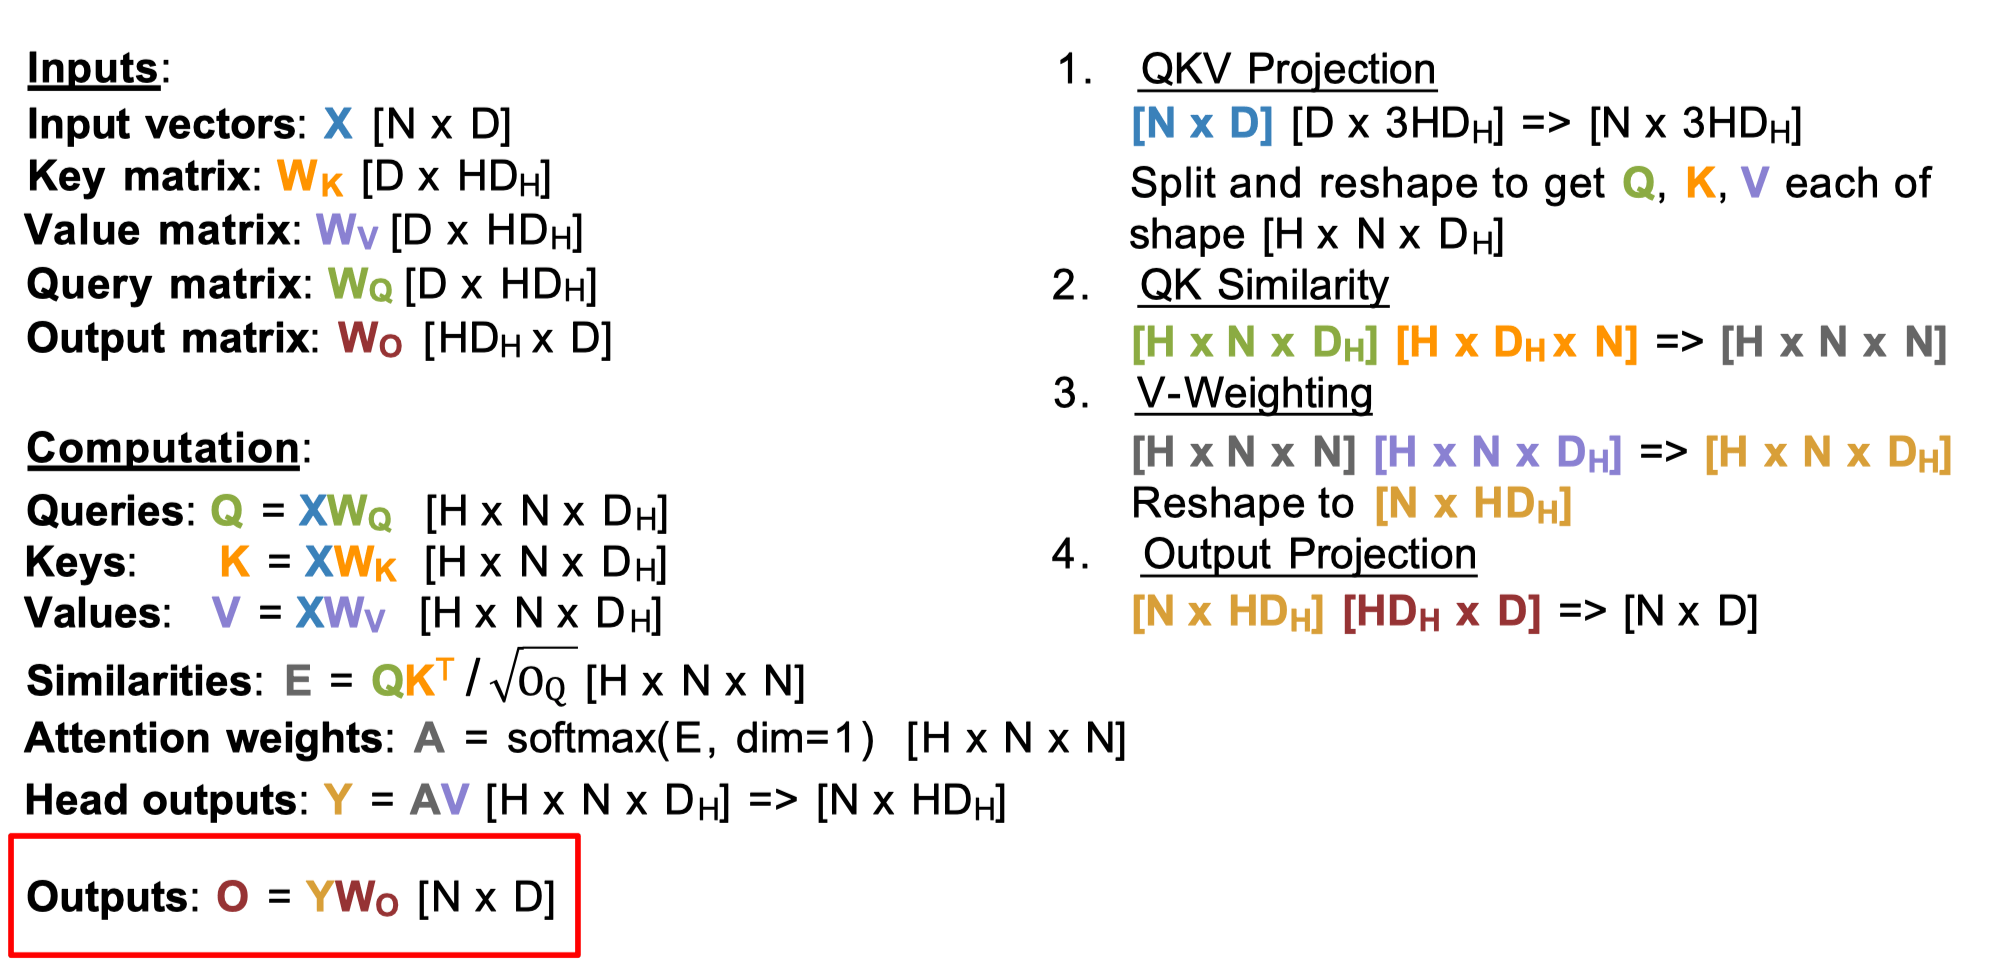
\includegraphics{./Cheatsheet-02-Self-Attention-and-Transformer.assets/image-20250617232437127.png}

\textbf{Masked Self-Attention / Causal
Attention}:用于解码器中,防止模型在预测当前位置时``看到''未来的信息。通过引入因果掩码,在计算注意力权重时将未来位置的分数设为
\(-\infin\),使其 Softmax 后的权重趋近于零。完美保证自回归因果性、结合了
CNN 的并行性与 RNN 的时序性。

\textbf{Multi-Head Attention}:将 Q, K, V
通过不同的线性变换投影到多个``头''(head),在每个头中独立计算注意力,然后将所有头的结果拼接并再次进行线性变换。\textbf{优点}:1.
允许模型从不同的表示子空间中学习信息(为每个头学习独立的
\(W_Q, W_K, W_V\) 矩阵),\textbf{表达能力更强};2.
\textbf{计算量与单头注意力基本相同}。

\textbf{三者比较}:\textbf{RNN} 的计算和空间复杂度均为
\(O(N)\),但无法并行。\textbf{CNN}
可并行,但感受野有限,不适合长序列,需多层堆叠才能捕捉长距离依赖,内在处理顺序。\textbf{Self-Attention}
适合长序列,可并行,具有全局感受野,本身不感知顺序(置换等变,需要位置编码),计算复杂度
\(O(N^2 \cdot D)\) (算 A、AV),空间复杂度 \(O(N^2)\) (存 A 做
Softmax)。Flash Attention 可将空间复杂度优化至
\(O(N)\),但计算复杂度不变。

\textbf{Transformer}:完全摒弃了 RNN 和
CNN,一个标准模块由\textbf{多头自注意力、残差连接与层归一化、前馈网络(FFN)、残差连接与层归一化堆叠}而成。自注意力层是唯一的向量间交互的地方,而
FFN 和 LayerNorm 对每个 Token 向量独立作用(沿 Token Dim
维度,\(\mu_i = \frac{1}{D} \sum_{j=1}^{D} h_{i,j}\),\(\delta_i = \sqrt{\frac{1}{D} \sum_{j=1}^{D} (h_{i,j} - \mu_i)^2 + \epsilon}\),\(z_i = \frac{h_i - \mu_i}{\delta_i}\),\(y_i = \gamma \odot z_i + \beta\),整个模型就是将这样的模块堆叠
L 次。

\textbf{Pre-Norm}:将层归一化(LayerNorm)移到自注意力和 FFN
\textbf{之前}(即残差连接的分支上),而不是之后。这使得训练过程更稳定,因为模型更容易学习恒等映射,\(y = x + \text{LN}(f(x))\)

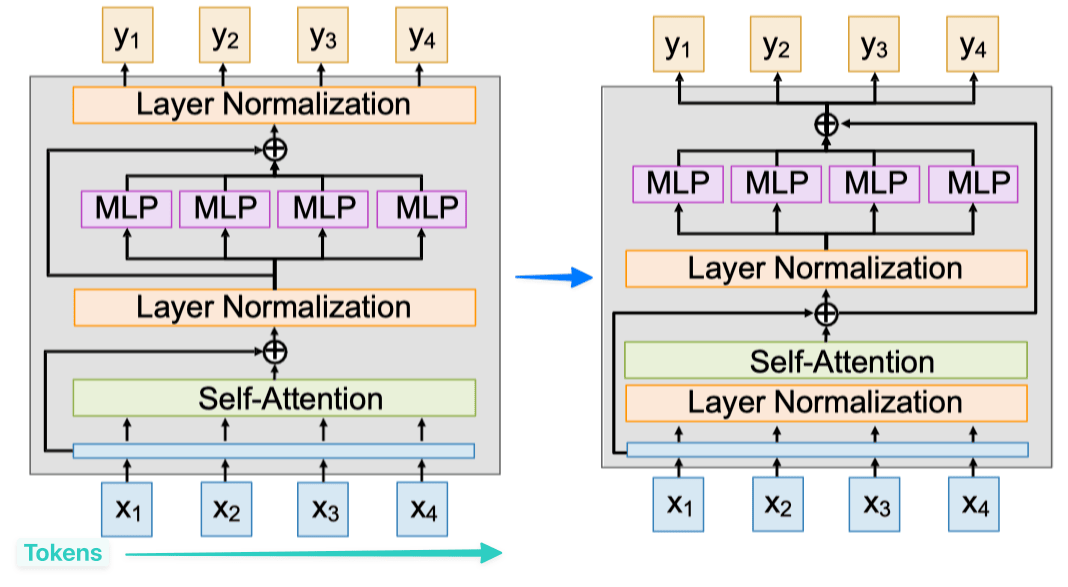
\includegraphics{./Cheatsheet-02-Self-Attention-and-Transformer.assets/image-20250618013153677.png}

\textbf{RMSNorm}:一种更简单、高效的归一化方法,替代 LayerNorm。公式为
\(y_i = \frac{x_i}{\sqrt{\varepsilon + \frac{1}{N} \sum_{i=1}^{N} x_i^2}} \cdot \gamma_i\)。它只缩放向量使其
Norm 一致,而不像 LN
那样进行中心化(类似让结果服从高斯分布),训练更稳定。

\textbf{SwiGLU}:一种改进的前馈网络(FFN/MLP)结构,性能优于标准
FFN。其结构为
\((\delta(\mathbf{X}\mathbf{W}_1) \odot \mathbf{X}\mathbf{W}_2)\mathbf{W}_3\),其中
\(\delta\) 为 Sigmoid/Swish,\(\odot\) 为逐元素乘法。设置 \(H = 8D/3\)
可以保持参数和 FFN(\(D \to 4D \to D\))相同。

\textbf{MoE}:在一个模块中训练 E 个独立的 FFN(专家),但对于每个输入
Token,只通过一个可学习的路由(Routing)机制选择 A 个(A \textless{}
E)专家进行计算。MoE 能以较小的计算成本(计算量提升 A
倍)实现巨大的模型参数量(参数量提升 E
倍),普遍采用。\textbf{训练挑战}:路由机制涉及不可导的选择操作,需平衡专家负载。\textbf{与标准
Transformer 比较}:1. 节省计算量(未路由到不参与计算);2.
更难训练(Topk 不可导)。

\textbf{ViT}:将图像分割成不重叠的小块
(Patches),每个块展平并线性投影成一个 Token,再加入 2D
\textbf{位置编码(学习得到)},送入标准 Transformer
编码器。图像任务中,所有 Token
之间可以互相关注,\textbf{无需掩码}。处理输出时,常对所有 Token
进行全局平均池化,再接线性层进行分类。

\textbf{多模态大模型}:本质是将不同来源的数据(文本、图像、声音等)都转化为统一的
\textbf{Token} 表示,然后用一巨大 Transformer 进行联合处理和学习。

\hypertarget{detection-segmentation}{%
\section{Detection \& Segmentation}\label{detection-segmentation}}

\textbf{CV
四大任务}:分类(图像整体类别)、语义分割(像素级分类,不区分同类实例,Dense
Prediction)、物体检测(识别并用框定位物体,但输出框的数量不确定)、实例分割(检测
+ 分割,像素级轮廓且区分实例)。

\textbf{物体检测}:定位 + 分类,输出平行于坐标轴的边界框(\textbf{理想要
tight}),4 自由度 \((x, y, h, w)\) / \((cx, cy, w, h)\)

\textbf{损失函数}:\(L_{total} = L_{cls} + \lambda L_{reg}\)。分类损失常用交叉熵;回归损失常用
Smooth L1 Loss。

\textbf{回归损失函数}:\textbf{L1}
\(\sum_{i \in \{x,y,w,h\}} |\hat{y_i} - y_i|\) 对异常值稳健但 0
点附近梯度不平滑,不利于模型在最优解附近精确收敛(震荡)。\textbf{L2}
\(\sum_{i \in \{x,y,w,h\}} (\hat{y_i} - y_i)^2\)
零点平滑但对异常值敏感,不等于 L2 Norm;\textbf{Smooth L1 Loss}
在误差小时似 L2 (保证平滑),误差大时似 L1
(控制梯度大小,稳健),分界点 \(x=\pm1\)
梯度平滑,是常用选择。\(\text {smooth}_{L_1}(x) = \begin{cases} 0.5x^2 & \text{if } |x| < 1 \\ |x| - 0.5 & \text{otherwise} \end {cases}\)。

\textbf{RMSE}
\(\sqrt {\frac {1}{N} \sum_{i \in \{x,y,w,h\}} (\hat {y_i} - y_i)^2}\),\textbf{优点}:单位与目标变量一致,易于理解;对大误差的敏感度介于
L1 和 L2 之间。\textbf{缺点}:在误差接近 0
时梯度会趋向无穷,可能导致数值不稳定;对异常值(因平方操作)仍然比较敏感;较
L1 计算仍然复杂。

\textbf{滑动窗口}:用不同尺寸的框暴力遍历图像,对每个框块运行分类器。计算量巨大,效率极低。

\textbf{R-CNN 系列
(两阶段)}:核心思想是先生成候选区域,再对区域进行分类和回归。

\textbf{R-CNN}:Selective Search 提议~2k RoIs \(\rightarrow\) 每个 RoI
独立缩放并送入 CNN 提特征 \(\rightarrow\) SVM 分类 +
选择性回归。\textbf{问题}:对每个 RoI 重复 CNN
前向传播,计算冗余极大,速度极慢;多阶段训练非端到端;信息损失(RoI
裁剪并变形),使得边界框回归(尤其先缩小然后扩大时)缺乏依据,丢失分辨率。

\textbf{Fast R-CNN}:\textbf{共享 CNN 提取特征的计算步骤},整图先过 CNN
得特征图 \(\rightarrow\) RoI 投影到特征图上 \(\rightarrow\) \textbf{RoI
Pooling} 将不同尺寸 RoI
转为固定尺寸特征向量(实现:划分,然后将点吸附(Snap)在子网格上,子网格内最大池化,输出固定尺寸)。\textbf{优点}:主体(除
SS 外)端到端。\textbf{缺点}:外部算法 \textbf{Selective Search}
成为速度瓶颈;RoI Pooling
两次量化会损失精度,前向提特征(以及预测类别)都还好说,反向还原求原图边界框的时候失去了空间信息不好做。

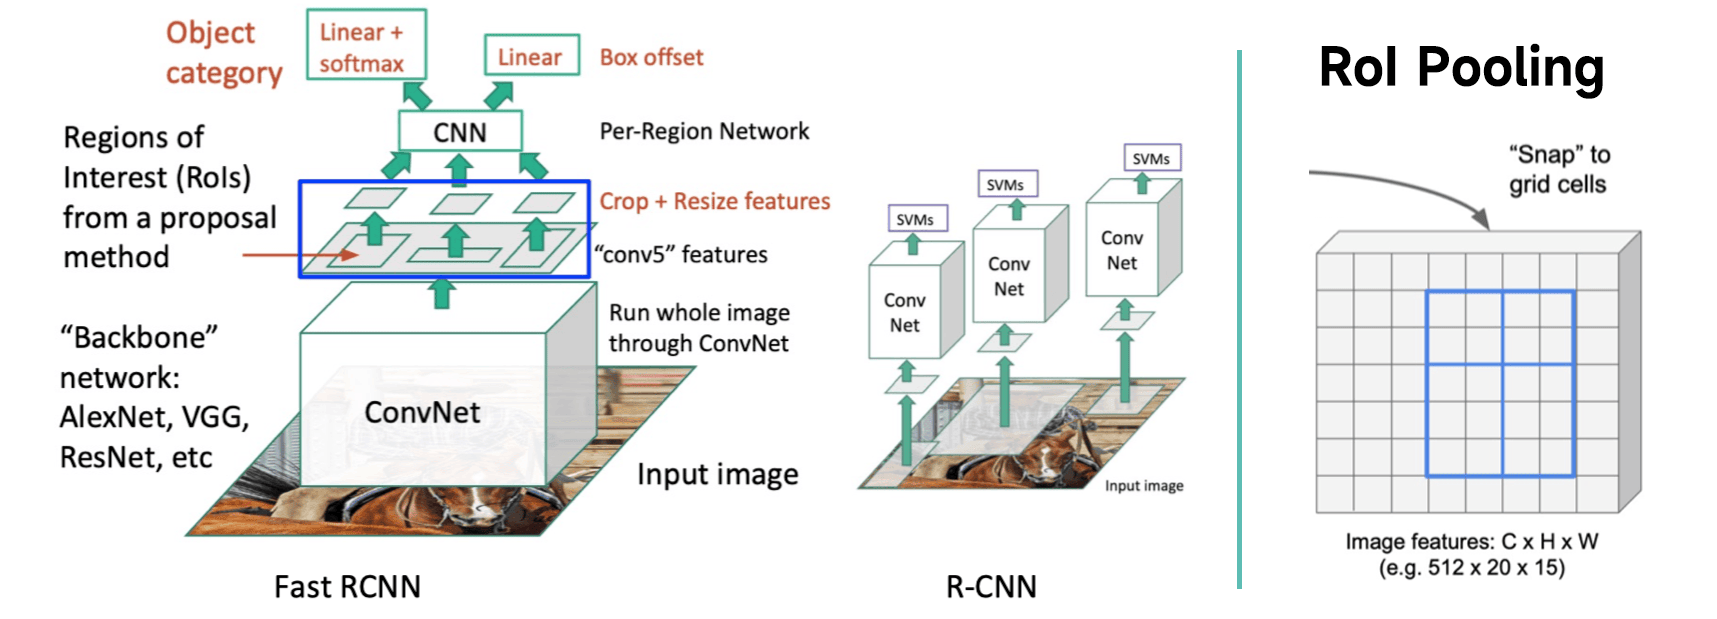
\includegraphics{./Cheatsheet-03-Detection-and-Segmentation.assets/image-20250618042307585.png}

\textbf{Faster R-CNN}:让网络自己学习生成候选区域。\textbf{区域提议网络
(Region Proposal Network,
RPN)},对主干特征图上的\textbf{每个点},使用一组预设尺寸、长宽比的
\textbf{锚框 (Anchor Boxes)} 预测 \textbf{Objectness Score} (前景 /
背景概率)和 \textbf{Box Refinement}
(边框微调),\textbf{在特征图上操作、全卷积很高效、可学习的}。\textbf{本质是一个两阶段检测器},阶段一(RPN)粗提候选框,阶段二
(检测头) 筛掉低阈值+NMS 后精细分类定位。\textbf{问题}:RPN 对分数进行
topk 操作引入不可导,训练复杂,包含 4 个损失函数(RPN 分类损失、RPN
回归损失、最终分类损失、最终回归损失),通常采用交替训练或联合训练的方式。

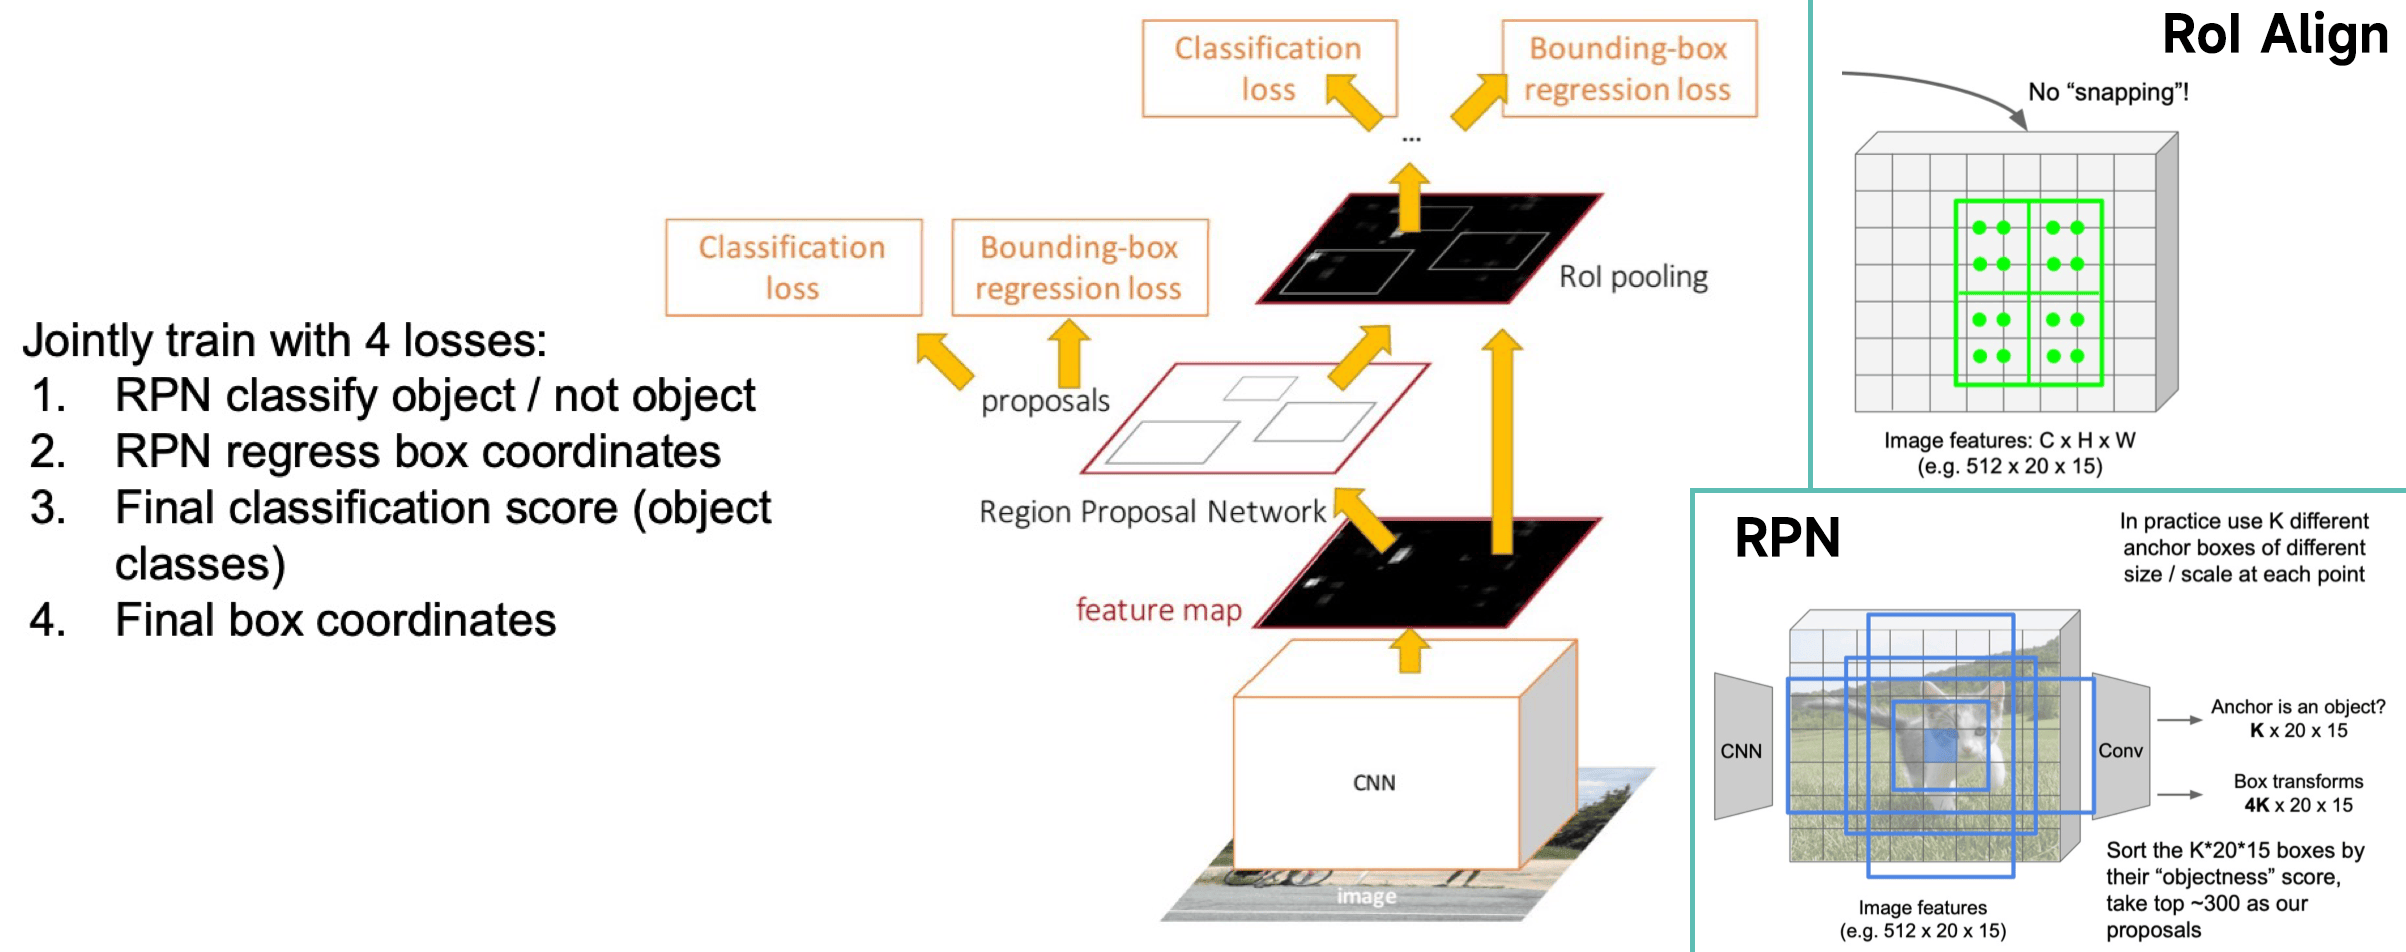
\includegraphics{./Cheatsheet-03-Detection-and-Segmentation.assets/image-20250618042701373.png}

\textbf{单阶段检测器
(YOLO)}:追求极致速度,一步到位。\textbf{核心思想}:将检测视为回归问题,将图像划分为粗糙网格,每个网格单元直接负责预测中心点落于此的物体的边界框和类别,本质是融合了
RPN
和检测头的功能。\textbf{优缺点}:速度极快,但早期版本精度和对小物体检测能力不如两阶段方法。

\textbf{NMS}:解决同一物体多个重叠检测框的问题。按置信度排序,保留最高分框,并移除与它
IoU \textgreater{}
阈值的其他框,迭代直至处理完所有框。\(\text{IoU} = \text{交集面积} / \text{并集面积}\)。注意
NMS \textbf{不可导}。

\textbf{评估指标}:\textbf{精确率 (Precision)}
\(\frac{TP}{TP+FP=Predict}\) (查准);\textbf{召回率 (Recall)}
\(\frac{TP}{TP+FN=GT}\) (查全)。\textbf{AP (平均精度)} 是单一类别 P-R(R
横轴,P 纵轴)曲线下的面积。\textbf{mAP (平均精度均值)} 是所有类别 AP
的均值,为标准评估指标。\textbf{AP 计算依赖 IoU
阈值},如\(AP_{50}/AP@50\),IoU 阈值越高,对定位的要求越严格,通常 PR
曲线会更靠左下方,AP 值会更低。

\textbf{画 PR 曲线}:注意因变量不是精确率也不是召回率,是按照 conf
排序选点 top k\% 的 k,可以出现锯齿。\textbf{11 点法}
\(AP \approx \frac{1}{11} \sum_{R \in \{0, 0.1, ..., 1.0\}} P(R)\),此时
\(P(R) = \max\{P(r)\ \text{for}\ r > R \}\),曲线单调递减。

\textbf{自顶向下
(Top-down)}:先检测,再分割。即先用目标检测器找到物体的边界框,然后在每个框内进行二元分割(前景/背景)\textbf{Mask
R-CNN} 是典型代表。

\textbf{自底向上
(Bottom-up)}:先分组,再分类。即先判断哪些像素属于同一个实例,将它们``簇''在一起形成掩码,然后再对每个掩码进行分类。

\textbf{Mask R-CNN}:在 Faster R-CNN
上并行增加掩码预测分支。核心创新是\textbf{RoI Align},解决 RoI Pooling
因两次量化取整导致的\textbf{空间错位 (Misalignment)}
这一对边框回归的巨大问题。

\textbf{RoI
Align}:取消硬性量化(避免取整),保留浮点坐标。当采样点不在特征图网格上时,使用\textbf{双线性插值}根据周围
4
个点计算其特征值,实现像素级对齐,极大提升掩码精度,得到精细边界,尤其在\textbf{高
IoU
阈值}(更严苛要求预测和真实轮廓重合)下。\(f_{xy} = \sum_{i,j=1}^{2} f_{i,j} \max(0, 1 - \lvert x - x_i \rvert) \max(0, 1 - \lvert y - y_j \rvert)\)

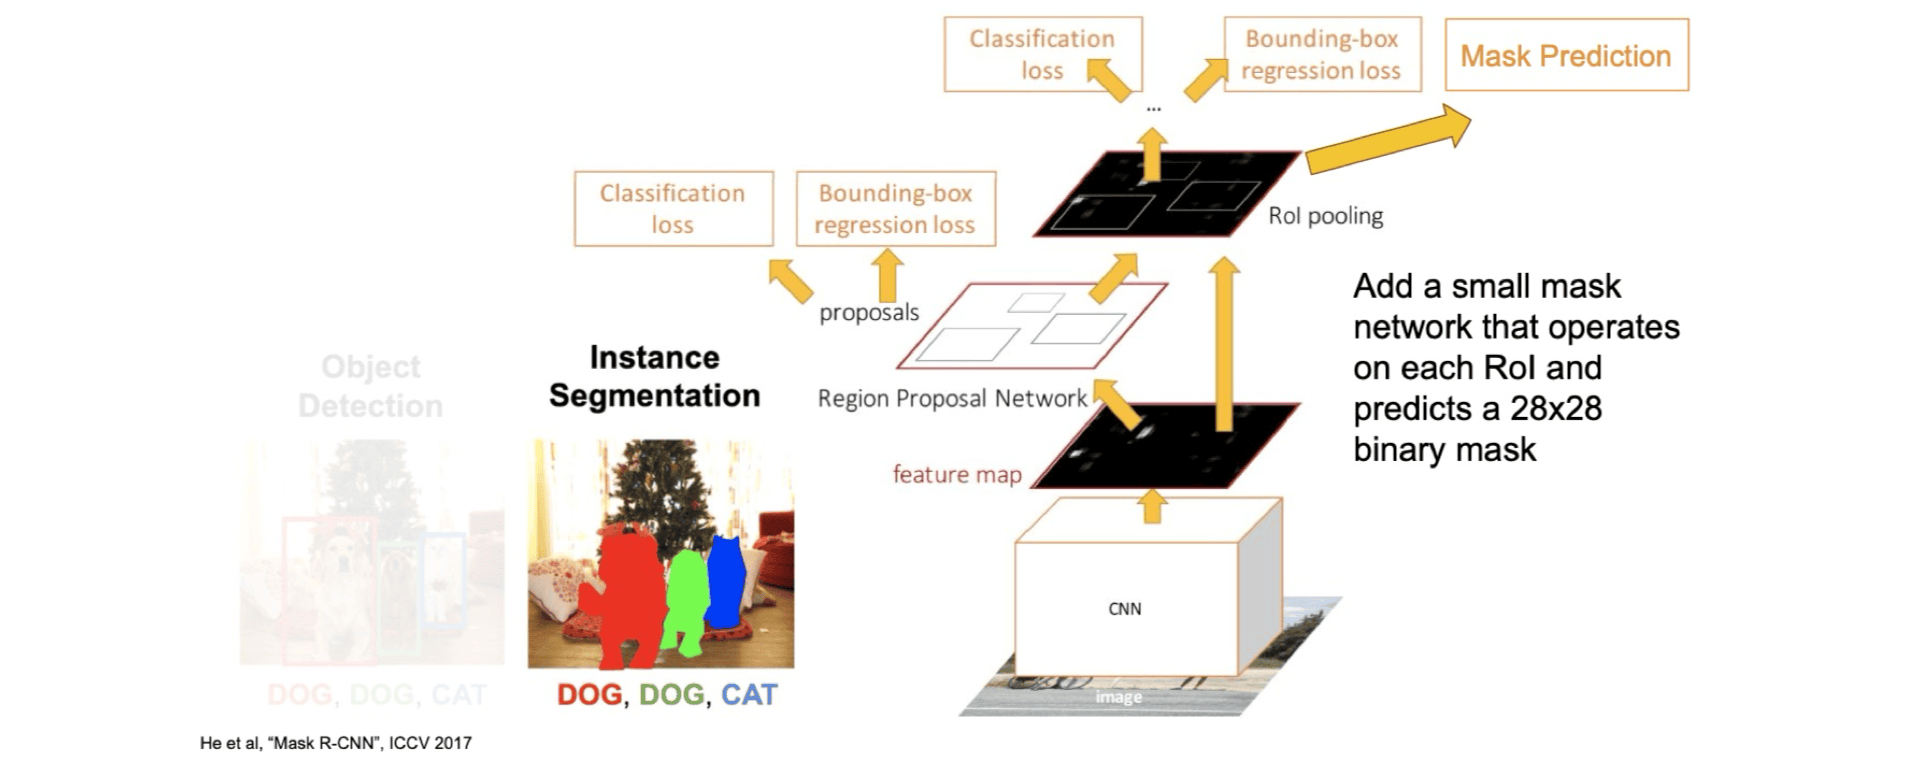
\includegraphics{./Cheatsheet-03-Detection-and-Segmentation.assets/image-20250618013701087.png}

\textbf{掩码设计}:\textbf{类别相关}:为每个类别都预测一个独立的掩码(例如,80个类=80个掩码输出,Mask
RCNN)。\textbf{类别无关}:只预测一个通用的``前景物体''掩码,类别由分类分支判断。\textbf{类别无关}(更简单)的方法效果与\textbf{类别相关}(更复杂)\textbf{几乎一样好},表明掩码形状预测与类别判断任务可以有效解耦。

\textbf{像素分类}:\textbf{多项式预测(Multinomial)}:对每个像素在所有类别间使用
\texttt{softmax},导致\textbf{类别间竞争},一个像素只能属于一个类别。\textbf{独立预测(Independent)}:对每个类别的掩码使用独立的\textbf{逐像素
\texttt{sigmoid}}
和二元损失。\textbf{没有类别间竞争},一个像素可以同时属于多个类的前景(处理重叠物体)。\textbf{独立预测显著优于多项式预测}。因为它解耦了类别预测,允许网络为每个类别独立学习其形状,而不会被其他类别干扰。

\textbf{3D目标检测}:通常输入为RGB-D或点云,自由度更高(如7
DoF:【x,y,z,w,h,l,yaw】)。\textbf{Frustum
PointNet}:利用2D检测结果生成视锥(Frustum),在视锥内的点云上进行3D分割和检测。高效但依赖2D,无法处理遮挡。\textbf{VoteNet}:受霍夫变换启发,让点云中的每个点``投票''给它可能属于的物体中心,通过聚合投票来定位物体。纯3D,但对小物体(表面点少投票不集中)、密集场景(不同点干扰)不好。

\hypertarget{generative-models}{%
\section{Generative Models}\label{generative-models}}

\textbf{目标}:学习一个模型分布 \(p_{\text{model}}(x)\)
来近似真实数据分布 \(p_{\text{data}}(x)\),\(x\) 可看做高维数据,\(p\)
是概率密度函数(连续化了,可以大于 1),并能从 \(p_{\text{model}}(x)\)
中采样新数据 \(x\)。\textbf{Explicit Density Model}:显式定义
\(p_{\text{model}}(x)\)。\textbf{Tractable(可处理)}:\(p_{\text{model}}(x)\)
可以被精确计算,或其对数似然可被高效优化。\textbf{Approximate}:\(p_{\text{model}}(x)\)
无法直接计算,需通过近似方法间接优化(VAE ELBO)。\textbf{Implicit
Density Models}:无需显式定义
\(p_{\text{model}}(x)\),直接学习采样过程(GAN)。生成模型不等于判别模型,学习数据的联合概率分布
\(P(X, Y)\) 或数据本身的分布 \(P(X)\)。

\textbf{不可能三角}:VAE 缺乏高质量样本(High Quality Samples);GAN
缺乏模式覆盖度/多样性(Mode Coverage/Diversity);Diffusion
缺乏快速采样(Fast Sampling)。

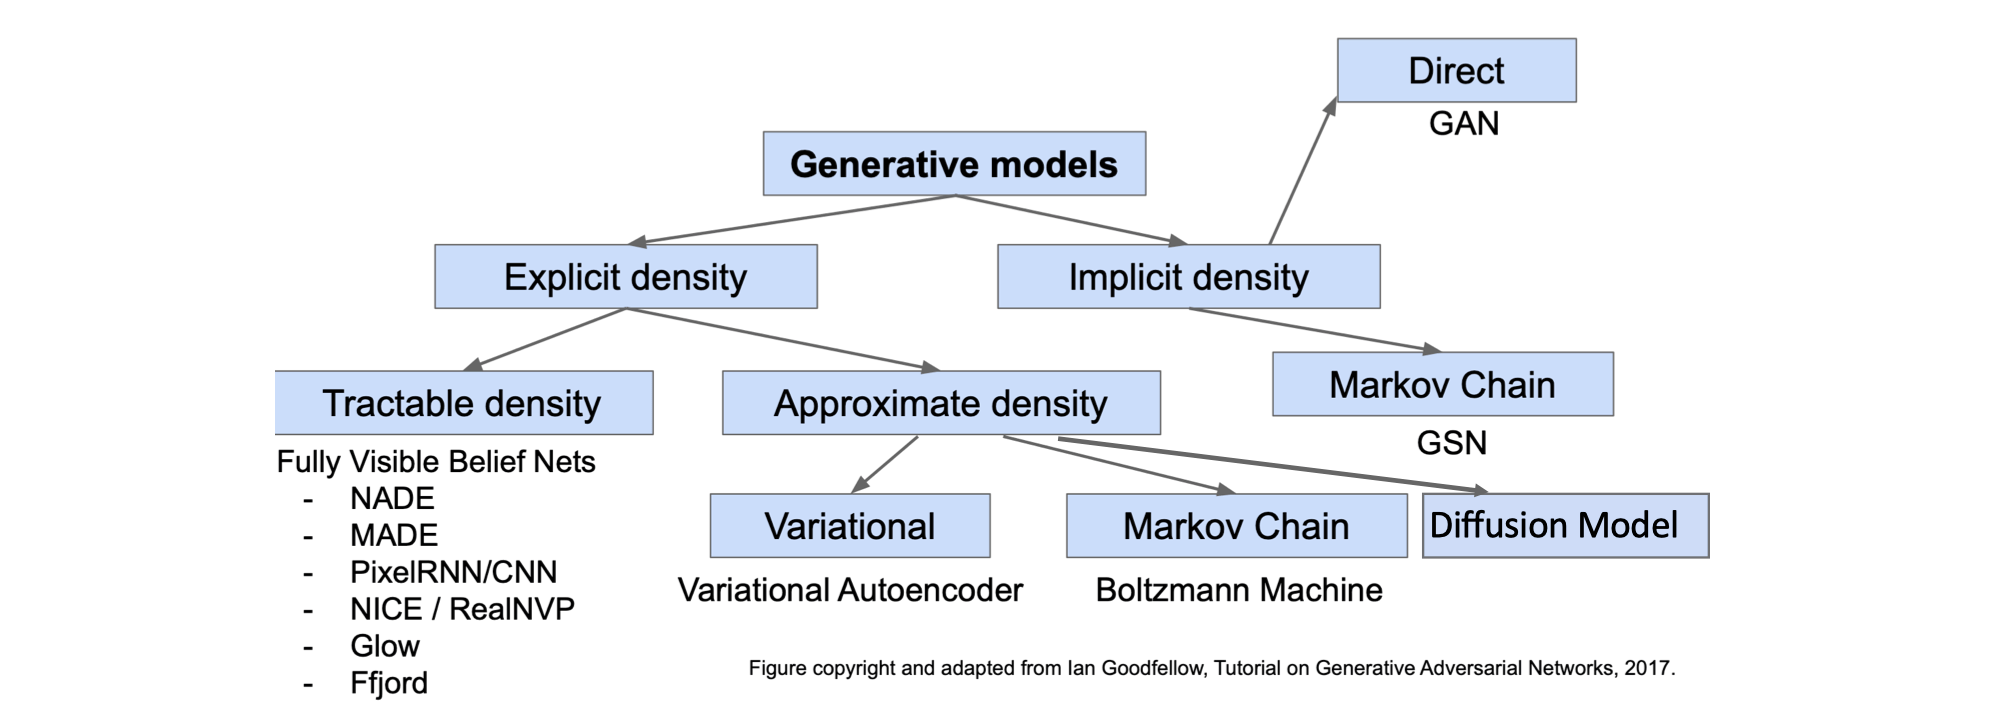
\includegraphics{./Cheatsheet-04-Generative-Model.assets/image-20250618013556902.png}

\textbf{Fully Visible Belief Network (FVBN)}:利用链式法则
\(p(x)=\prod p(x_i | x_{<i})\),将联合概率拆解为``第 i
个像素值在给定所有先前像素下的概率''的乘积。通过最大化训练数据的
\(p(x)\) 来训练,例如 PixelRNN(可见副对角线以上区域) 和
PixelCNN(可见左上区域)。\textbf{优点}:可以显式计算似然函数
\(p(x)\),生成高质量样本,容易优化。\textbf{缺点}:生成过程必须按顺序进行(\textbf{自回归}),速度较慢,且不符合直觉。

\textbf{Autoencoder(AE) }:将输入 \(x\) 映射到唯一确定的隐变量
\(z\)(不建模概率),无法从 \(z\) 空间采样生成,有效的 \(z\)
实际是空间中的流形(manifold),在整个 \(z\) 空间中可能极其微小。

\textbf{Variational Autoencoders (VAE)}:将 \(x\)
编码为一个概率分布,并强制整个隐空间服从一个易于采样的先验分布(标准正态分布
\(\mathcal{N}(0, I)\)),学复杂的条件分布 \(p(x|z)\)。核心思想是用一个
Encoder \(q_\phi(z|x)\) 来近似棘手的真实后验分布
\(p_\theta(z|x)\)。训练时优化的不是真实对数似然
\(\log p_\theta(x) = \log \int p_\theta(x|z)p(z)dz\)(积分导致
Intractable),而是其下界,ELBO。

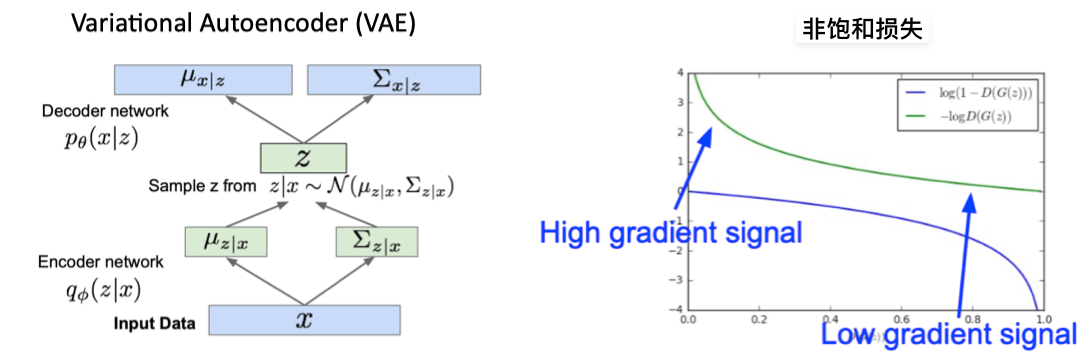
\includegraphics{./Cheatsheet-04-Generative-Model.assets/image-20250617192929555.png}

\textbf{ELBO}
\(L(x^{(i)}, \theta, \phi) = E_z[\log p_\theta(x^{(i)}|z)] - D_{KL}(q_\phi(z|x^{(i)}) || p(z))\)。

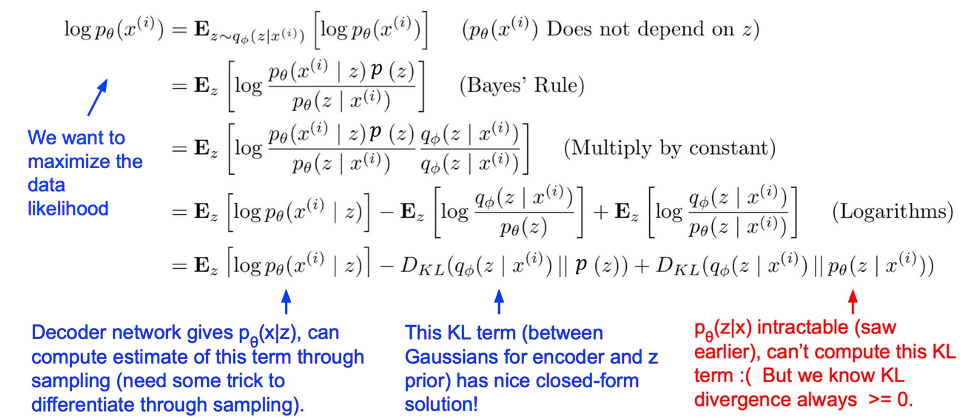
\includegraphics{./Cheatsheet-04-Generative-Model.assets/image-20250617192057785.png}

第一项是\textbf{重建项},最大化给定潜变量 \(z\)
时原始输入被重建的似然(实践中常扔掉方差项,简化为 L2 损失
\(||x - \mu_{x|z}||^2\));第二项是\textbf{正则项},使近似后验 \(q\)
与先验 \(p(z)\) 尽可能接近。\textbf{核心矛盾}:重建项希望编码精确,KL
项希望编码趋同,二者的拉扯导致 VAE
生成的图像较为\textbf{模糊}。\textbf{Intractable 问题}:ELBO 中的期望
\(E_z\) 仍是 \textbf{Intractable 棘手的},需用蒙特卡洛方法采样 \(z\)
来估计。\textbf{重参数化技巧}:前向 encoder 从 \(q_\phi(z|x)\) 中采样
\(z\) 的步骤是随机的,这会导致梯度无法回传。解决:训练时从
\(\mathcal{N}(0, I)\) 中采样 \(\epsilon\),结合 encoder
输出的均值和方差得到
\(z = \mu_{z|x} + \epsilon \sigma_{z|x}\),使梯度能够反向传播。\textbf{推理
(Sampling)}:直接从先验分布 \(p(z)\) 中采样
\(z\),再通过解码器生成样本。\textbf{优点}:生成模型的原理性方法;提供可解释的潜空间;可进行
\(q(z|x)\)
的推理用于其他任务,可插值观察到平滑变化(学习到了一个有意义且连续的隐空间,解耦了各主要变化因素)。\textbf{缺点}:优化的是下界,生成样本质量不如
GAN 和 Diffusion(MSE 导致倾向于平均化预测,失去高频细节)。

\textbf{Generative Adversarial Networks
(GAN)}:\textbf{隐式密度}生成模型,包含一个生成器 (Generator)
和一个判别器 (Discriminator),二者进行博弈。\textbf{目标函数}
\(\min_{\theta_g} \max_{\theta_d} [E_{x \sim p_{\text{data}}} \log D_{\theta_d}(x) + E_{z \sim p(z)} \log(1 - D_{\theta_d}(G_{\theta_g}(z)))]\)。\textbf{训练伪码}:每轮迭代,判别器(真实+生成数据监督)可先梯度反传
\(k\) 次(\(k \ge 1\)),生成器再反传一次(仅生成数据监督)。

\textbf{生成器非饱和损失 (Non-saturating Loss)}:实践中,最小化
\(E_{z \sim p(z)} \log(1 - D(G(z)))\)(蓝色曲线)在早期\textbf{梯度消失},效果不好,因此改为最大化
\(E_{z \sim p(z)} \log(D(G(z)))\)(绿色曲线)。

\textbf{DCGAN 架构改进}:用步长卷积/分数步长卷积替换池化层;使用 BN
稳定数据分布;移除全连接层;生成器用 ReLU(输出层用 Tanh),判别器用
LeakyReLU。

\textbf{定性评估}:Nearest neighbors
对比生成样本与训练集最近邻,检测过拟合;User Study
让人类判断真伪。\textbf{定量评估}:Fréchet Inception Distance (FID)
将真实和生成样本集通过 Inception Net 提取特征,分别计算特征分布的均值
\(\mu\) 和协方差 \(\Sigma\),再用公式
\(FID(r, g) = ||\mu_r - \mu_g||_2^2 + \text{Tr}(\Sigma_r + \Sigma_g - 2(\Sigma_r \Sigma_g)^{1/2})\)
计算距离。\textbf{FID
分数越低,表示生成图像的质量和多样性越接近真实图像}。FID
对图像失真(如噪声、模糊)非常敏感。

\textbf{Mode Drop/Collapse
模式崩溃}:生成器只学会了数据分布中可以骗过判别器的少数几个模式,无法覆盖多样性。

\textbf{优点}:生成样本质量高且美观(偏好多样性小、数据量大的情况),\textbf{可以进行语义向量运算/可解释性}。\textbf{缺点}:训练困难且不稳定;容易模式崩溃导致多样性不足;无法解决推断查询(Inference
Queries)/概率推断,即计算 \(p(x)\) 或 \(p(z|x)\) 并基于此回答问题。

\textbf{Diffusion Model}:思想源于分层 VAE,可视为具有 T
个潜变量的特例(马尔科夫链),其独特之处在于前向过程固定无参数,且最终潜变量被设计为收敛到标准高斯分布。\textbf{前向加噪}:一个固定无需学习的马尔可夫链,在
T 步中逐渐向真实数据 \(x_0\) 添加高斯噪声,最终得到
\(x_T \sim \mathcal{N}(0, I)\)。\textbf{反向去噪}:学习一个神经网络来逆转加噪过程,从纯噪声
\(x_T\) 出发,逐步去除噪声,最终恢复出图像 \(x_0\)。

\textbf{训练目标}:在实践中被简化为反向时预测前向所加噪声。随机采样
\(x_0\) 和时间步 \(t\),生成加噪图 \(x_t\),然后训练去噪网络
\(\epsilon_\theta\) 预测在第 \(t\) 步加入的真实噪声
\(\epsilon\),损失函数通常为预测噪声与真实噪声间的均方误差
MSE。\(L = \mathbb{E}_{x_0, \epsilon, t} [||\epsilon - \epsilon_\theta(\sqrt{\bar{\alpha}_t}x_0 + \sqrt{1-\bar{\alpha}_t}\epsilon, t)||^2]\)。\textbf{可控条件生成}:通过引入条件信息
\(y\)(如文本),可实现强大的可控生成。\textbf{优点}:高质量、高多样性、条件生成灵活可控;\textbf{缺点}:采样速度慢,现用
DDIM 加速。

\end{multicols*}

\end{document}
